\documentclass[runningheads,a4paper]{llncs}

% ---- Packages ----
\usepackage{makeidx}
\usepackage{graphicx}
\usepackage[neverdecrease]{paralist}
\usepackage{fancyvrb}
\usepackage{multirow}
\usepackage{tabularx}
\usepackage{url}
\usepackage{amsmath}
\usepackage[LGRgreek]{mathastext}
\usepackage{enumitem}
\usepackage{array}
\usepackage{chngcntr}
\usepackage{centernot}
\usepackage{algorithmic}
\usepackage{mathtools}
\DeclarePairedDelimiter{\ceil}{\lceil}{\rceil}
\usepackage{titletoc}
\usepackage[ruled,noend,noline,slide]{algorithm2e}


% ---- Settings ----

% --- Margins ---
%\usepackage{fullpage}
%\usepackage[margin=1.25 in]{geometry}

% --- Appendix settings ---
\usepackage[title,titletoc,header]{appendix}
\makeatletter
\newcommand{\@chapapp}{\relax}%
\makeatother

% --- Running header settings ---
\usepackage{fancyhdr}
\pagestyle{fancy}
\renewcommand{\sectionmark}[1]{ \markright{#1} }
\newcommand{\titlemark}{ Bitcoin Developer Reference }
\newcommand{\bibmark}{ Bibliography }

\fancyhf{}
\fancyhead[LE,RO]{\bfseries\thepage}
\fancyhead[LO]{\bfseries\rightmark} % Odd pages, section name printed
\fancyhead[RE]{\bfseries\titlemark} % Even pages
\renewcommand{\headrulewidth}{0.5pt}
\renewcommand{\footrulewidth}{0pt}
\addtolength{\headheight}{0.5pt}
\fancypagestyle{plain}{
	\fancyhead{}
	\renewcommand{\headrulewidth}{0pt}
}

% --- Figure and Table numbering ---
\counterwithin{figure}{section}
\counterwithin{table}{section}

% --- Custom table settings ---
\newcolumntype{C}[1]{ >{\centering\arraybackslash\smallskip} m{#1}<{\smallskip} }

\newcommand{\bigcell}[2]{\begin{tabular}{@{}#1@{}}#2\end{tabular}}
\def\tabularxcolumn#1{m{#1}}

% --- Custom list settings ---
\newlength{\wideitemsep}
\setlength{\wideitemsep}{.5\itemsep}
\addtolength{\wideitemsep}{5pt}
\let\olditem\item
\renewcommand{\item}{\setlength{\itemsep}{\wideitemsep}\olditem}


\begin{document}

% ---- Make a proper TOC despite llncs ----
\setcounter{tocdepth}{3}
\setcounter{secnumdepth}{3}
\makeatletter
\renewcommand*\l@author[2]{}
\renewcommand*\l@title[2]{}
\makeatletter



\title{Bitcoin Developer Reference}
\subtitle{Working Paper\\Last changes: \today}

\author{Krzysztof Okupski}

\institute{Technische Universiteit Eindhoven, The Netherlands\\
\email{k.s.okupski@student.tue.nl}}



%%%----------------------------------------------------------
\frontmatter
\maketitle

\clearpage
\tableofcontents
%%%----------------------------------------------------------



%%%----------------------------------------------------------
\mainmatter         % Main matter
%%%----------------------------------------------------------

\section{Introduction} \label{sec:Introduction}
Bitcoin is a decentralized digital cryptocurrency created by pseudonymous developer Satoshi Nakamoto. The first paper on Bitcoin \cite{Nakamoto_Bitcoin}, also referred to as the original Bitcoin paper, was published by Nakamoto in 2008. It provides a brief description of the concepts and architecture schematics of the Bitcoin protocol. It was used as theoretical groundwork for the first implementation of a fully functional Bitcoin client. However, up until now, no structured and accessible protocol specification has been written. Although the Bitcoin community has successfully created a protocol specification \cite{Wikipedia_ProtocolSpec}, it requires solid prior understanding of its concepts and implementation. In this paper a formal and accessible specification of the core Bitcoin protocol, i.e. excluding the P2P overlay network, will be presented.
\section{Preliminaries} \label{sec:Preliminaries}
This section gives a short introduction to cryptographic constructs necessary for a thorough understanding of the protocol. In particular, the proof-of-work scheme and Merkle trees will be discussed. Note that Digital Signatures are required as well but are intentionally skipped for they are sufficiently covered by online literature.

\subsection{Proof of Work} \label{sec:ProofOfWork}
A proof-of-work is a cryptographic puzzle used to ensure that a party has performed a certain amount of work. In particular, the Bitcoin mining process (see Sect. \ref{sec:Mining}) incorporates a proof-of-work system based on Adam Back's Hashcash \cite{Back_Hashcash}. It has two basic properties - firstly, it ensures that the party providing the proof-of-work has invested a predefined amount of effort in order to create the proof and secondly, that the proof is efficiently verifiable. Typically, finding a solution proof-of-work puzzle is a probabilistic process with a success probability depending on the predefined difficulty.

Let Alice and Bob be two parties communicating with each other and let Alice require Bob to perform a certain amount of computational work for each message he sends to Alice. To do so, Alice can require Bob to provide a string whose one-way hash satisfies a predefined structure. Finding such a string has a certain success probability that will determine how much work Bob has to invest on average in order to find a valid solution.

For example, in Bitcoin the hashing algorithm is \emph{double-SHA256} ($\mathit{SHA256^{2}}$) and the predefined structure is a hash less or equal to a target value \emph{T}. The success probability of finding a nonce \emph{n} for a given message \emph{msg}, such that $\mathit{H = SHA256^{2}(msg||n)}$ is less or equal to the target \emph{T} is
\begin{equation}
Pr[H \leq T] = \frac{T}{2^{256}}.
\end{equation}

\newpage
\noindent
This will require a party attempting to find a proof-of work to perform, on average, the following amount of computations
\begin{equation}
\frac{1}{Pr[H \leq T]} = \frac{2^{256}}{T}.
\end{equation}

\noindent
Finally, it is easy to see that it can be efficiently verified whether the nonce accompanied with the message is indeed a valid proof-of-work by simply evaluating
\begin{equation}
SHA256^{2}(msg||n) \leq T.
\end{equation}


\subsection{Merkle Trees} \label{sec:MerkleTrees}
Merkle trees, named after their creator Ralph Merkle, are binary hash trees used for efficient verification of data integrity. An example of a Merkle tree can be seen in Fig. \ref{fig:MerkleTree}. Leaves are computed directly as hashes over data blocks, whereas nodes further up the tree are computed by concatenating and hashing their respective children.

\begin{figure}[htbp]
 \centering
 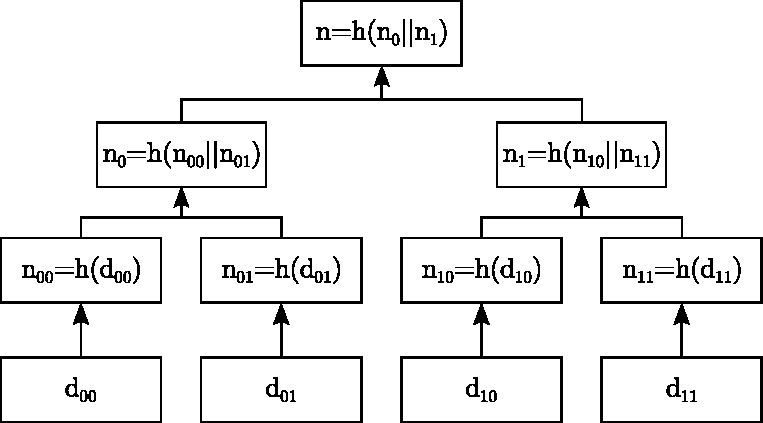
\includegraphics[scale=0.75]{images/MerkleTree.pdf}
 \caption{Merkle Tree}
 \label{fig:MerkleTree}
\end{figure}
\vspace{-10pt}

\noindent
The main advantage of Merkle trees is that when one data block changes it is not necessary to compute a hash over all the data, as opposed to naive hashing. Assume data block $\mathit{d_{00}}$ is modified, then $\mathit{n_{00}}$ has to be re-computed as well as all nodes along the branch until the root node. Therefore, the number of required hash computations scales logarithmically in the number of data blocks. Since both data blocks and hashes are relatively small in size, this process is fairly efficient.

\subsubsection*{Other cases}
The previously discussed example considered the situation where the number of data blocks is a power of two. In such a case the computation results in a full and complete binary tree. However, since it is required that each node, except for the leaves, has exactly two children, measures have to be taken if nodes are missing. In the following the method used in Bitcoin will be discussed.

\noindent
The solution is straightforward - when forming a row in the tree (excluding the root), whenever there is an odd number of nodes, the last node is duplicated. In effect, each intermediary row in the tree will always have an even number of nodes and therefore each node, except for the leaves, will have exactly two children.

\begin{figure}[htbp]
 \centering
 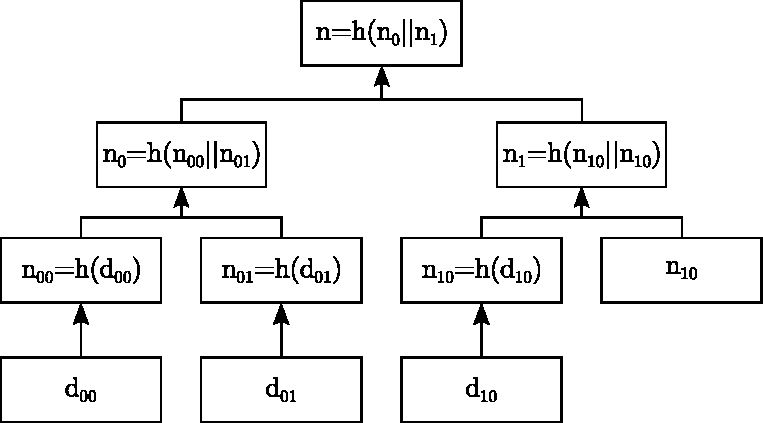
\includegraphics[scale=0.75]{images/MerkleTree2.pdf}
 \caption{Merkle Tree with Missing Nodes}
 \label{fig:MerkleTree2}
\end{figure}
\vspace{-10pt}

\noindent
In the example given in Fig. \ref{fig:MerkleTree2} there are only three data blocks and therefore the computation of the fourth node in the second row is missing a child. Thus, the last node is replicated and the computation is continued as in the previous example (see Fig. \ref{fig:MerkleTree}). Should an odd number of nodes occur at any other point during the computation, then the same rule is applied.

\clearpage
\section{Architecture} \label{sec:Architecture}
Central to Bitcoin's architecture is a public ledger called the \emph{blockchain}, which stores all processed \emph{transactions} in chronological order. Transactions are processed by a loosely-organized network of \emph{miners} in a process called \emph{mining} (see Sect. \ref{sec:Mining}). In it the miner creates a block with a set of unprocessed transactions and attempts to solve a proof-of-work puzzle (see Sect. \ref{sec:ProofOfWork}). Once a valid solution has been found, the block including the solution is published throughout the network and accepted into the blockchain. In this section the structure of blocks and transactions will be discussed in detail. Note that the following description is based on the Bitcoin source code \cite{BitcoinSourceCode} and the Bitcoin Protocol Specification on Wikipedia \cite{Wikipedia_ProtocolSpec}. Furthermore, all data types denoted in the diagrams are explained in detail in \ref{sec:DataTypes}.

\subsection{Blocks} \label{sec:Blocks}
Each block is composed of a header and a payload. The header stores the current block header version (\textit{nVersion}), a reference to the previous block (\textit{HashPrevBlock}), the root node of the Merkle tree (\textit{HashMerkleRoot}), a timestamp (\textit{nTime}), a target value  (\textit{nBits}) and a nonce (\textit{nNonce}). Finally, the payload stores transactions included in the block.

\begin{table}[ht!]
	\begin{tabularx}{\textwidth}{ | m{70pt} | >{\centering} m{60pt} | X |}

		\hline
		\textbf{Field name} &
		\bigcell{c}{\textbf{Type} \\ \textbf{(Size)}} &
		\textbf{Description}\\ \hline\hline
    
		nVersion &
		\bigcell{c}{int \\ (4 bytes)} &
		Block format version (currently 2). \\ \hline
		
		HashPrevBlock &
		\bigcell{c}{uint256 \\ (32 bytes)} &
		Hash of previous block header \newline
		$SHA256^{2}(nVersion || \dots || nNonce)$. \\ \hline
	
		HashMerkleRoot &
		\bigcell{c}{uint256 \\ (32 bytes)} &
		Top hash of the Merkle tree built from all transactions. \\ \hline
		
		nTime &
		\bigcell{c}{unsigned int \\ (4 bytes)} &
		Timestamp in UNIX-format of approximate block creation time. \\ \hline
	
		nBits &
		\bigcell{c}{unsigned int \\ (4 bytes)} &
		Target T for the proof-of-work problem in compact format. Full target value is derived as:\newline$T = 0xh_{2}h_{3}h_{4}h_{5}h_{6}h_{7} * 2^{8*(0xh_{0}h_{1} - 3)}$\\ \hline
	
		nNonce &
		\bigcell{c}{unsigned int \\ (4 bytes)} &
		Nonce allowing variations for solving the proof-of-work problem.\\ \hline
	
		\#vtx &
		\bigcell{c}{VarInt \\ (1-9 bytes)} &
		Number of transaction entries in \textit{vtx}. \\ \hline
	
		vtx[\,] &
		\bigcell{c}{Transaction \\ (Variable)} &
		Vector of transactions. \\ \hline
	\end{tabularx}
	\vspace{5pt}
	\caption{Block Structure Description}
	\label{table:CBlock}
\end{table}

\vspace{-30pt}
\clearpage

\subsubsection*{nVersion}
The version field stores the version number of the block format. Ever since BIP0034 \cite{BIP0034} is in place, the block format version is 2 and blocks of any other version are neither relayed nor mined.

\subsubsection*{HashPrevBlock}
This field stores the reference to the previous block, computed as a hash over the block header as depicted in Fig. \ref{fig:HashPrevBlock}.
\begin{figure}[ht!]
 \centering
 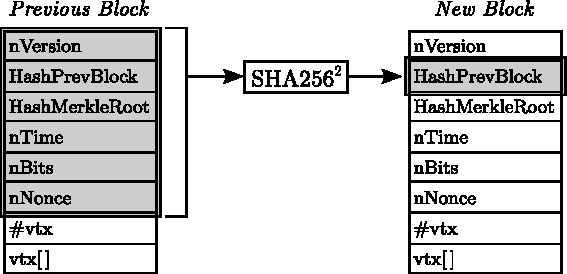
\includegraphics[scale=0.9]{images/HashPrevBlock.pdf}
 \caption{Block Reference Computation} \label{fig:HashPrevBlock}
\end{figure}

\noindent
A double-SHA256 hash is calculated over the concatenation of all elements in the previous block header:
\begin{equation}
\begin{aligned}
SHA256^{2}(nVersion||HashPrevBlock||HashMerkleRoot||nTime||nBits||nNonce)
\label{eqn:HashPrevBlock}
\end{aligned}
\end{equation}

\noindent
The reference functions as a chaining link in the blockchain. By including a reference to the previous block, a chronological order on blocks, and thus transactions as well, is imposed.


\subsubsection*{HashMerkleRoot}
This field stores the root of the Merkle hash tree. It is used to provide integrity of all transactions included in the block and is computed according to the scheme described in Sect. \ref{sec:MerkleTrees}. The parameters used for computing the tree are double-SHA256 as the hashing algorithm and raw transactions as data blocks (see Table \ref{tab:TransactionRegular} and \ref{tab:TransactionCoinbase}).


\subsubsection*{nTime}
The time field stores the timestamp in UNIX format denoting the approximate block creation time. As the timestamp is a parameter included in block mining, it is fixed at the beginning of the process.


\subsubsection*{nBits}
The \textit{nBits} field stores a compact representation of a target value \emph{T}, which is utilized in the proof-of-work puzzle (see Sect. \ref{sec:Mining}). The target value is a 256 bit long number, whereas its corresponding compact representation is only 32 bits long and thus encoded with only 8 hex digits. The target value can be derived from its compact hexadecimal representation $\mathit{0xh_{0}h_{1}h_{2}h_{3}h_{4}h_{5}h_{6}h_{7}}$ with the formula:
\begin{equation}
0xh_{2}h_{3}h_{4}h_{5}h_{6}h_{7} * 2^{8*(0xh_{0}h_{1} - 3)}
\end{equation}


\noindent
The upper bound for the target is defined as $\texttt{0x1D00FFFF}$ whereas there is no lower bound. The very first block, the genesis block, has been mined using the maximum target. In order to ensure that blocks are mined at a constant rate of one block per 10 minutes throughout the network, the target \emph{T} is recalculated every 2016 blocks based on the time $\mathit{t_{sum}}$ it took to mine, due to an off-by-one error \cite{nBitsCalc}, the last 2015 blocks:
\begin{equation}
T' = \dfrac{t_{sum}}{14*24*60*60s}*T
\end{equation}

\noindent
Note that $\mathit{t_{sum}}$ is calculated as the difference of the timestamps \textit{nTime} in the block header.

\subsubsection*{nNonce}
The nonce field contains arbitrary data and is used as a source of randomness for solving the proof-of-work problem. However, since it is fairly small in size with 4 bytes, it does not necessarily provide sufficient variation for finding a solution. Therefore, other sources exist and will be addressed in more detail in Sect. \ref{sec:Mining}.


\clearpage
\subsection{Transactions} \label{sec:Transactions}
In principle, there are two types of transactions - coinbase transactions and regular transactions. Coinbase transactions are special transactions in which new Bitcoins are introduced into the system. They are included in every block as the very first transaction and are meant as a reward for solving a proof-of-work puzzle. Regular transactions, on the other hand, are used to transfer existing Bitcoins amongst different users. From an architectural point of view, a coinbase transaction can be seen as a special case of a regular transaction. For this reason, the structure of a regular transaction will be discussed first, followed by the differences between coinbase and regular transactions.

\enlargethispage{2\baselineskip}
\subsection*{Regular transactions} \label{sec:RegularTransactions}
As mentioned in the previous section, each block in the blockchain includes a set of transactions. Every transaction consists of a transaction version (\textit{nVersion}), a vector of inputs (\textit{vin}) and a vector of outputs (\textit{vout}), both preceded by their count, and a transaction inclusion date (\textit{nLockTime}).
\begin{table}[ht!]
	\begin{tabularx}{\textwidth}{ | m{25pt} | m{70pt} | >{\centering} m{60pt} | X |} \hline
		\multicolumn{2}{|l|}{\textbf{Field name}} &
		\bigcell{c}{\textbf{Type} \\ \textbf{(Size)}} &
		\textbf{Description}\\ \hline\hline
    	
    	\multicolumn{2}{|l|}{nVersion} &
    	\bigcell{c}{int \\ (4 bytes)} &
    	Transaction format version (currently 1).\\ \hline
    	
	    \multicolumn{2}{|l|}{\#vin} &
	    \bigcell{c}{VarInt \\ (1-9 bytes)} &
    	Number of transaction input entries in \textit{vin}. \\ \hline
    	
		\multirow{9}{25pt}{\centering vin[\,]} &
		
		hash &
		\bigcell{c}{uint256 \\ (32 bytes)} &
		Double-SHA256 hash of a past transaction.\\ \cline{2-4}
		
		& n &
		\bigcell{c}{uint \\ (4 bytes)} &
		Index of a transaction output within the transaction specified by \textit{hash}. \\ \cline{2-4}

		& scriptSigLen &
		\bigcell{c}{VarInt \\ (1-9 bytes)} &
		Length of \textit{scriptSig} field in bytes. \\ \cline{2-4}
				
		& scriptSig &
		\bigcell{c}{CScript \\ (Variable)} &
		Script to satisfy spending condition of the transaction output (\textit{hash},\textit{n}). \\ \cline{2-4}
		
		& nSequence &
		\bigcell{c}{uint \\ (4 bytes)} &
		Transaction input sequence number. \\ \hline
    	
    	\multicolumn{2}{|l|}{\#vout} &
	    \bigcell{c}{VarInt \\ (1-9 bytes)} &
    	Number of transaction output entries in \textit{vout}. \\ \hline
    	
		\multirow{5}{25pt}{\centering vout[\,]} &
		
		nValue &
		\bigcell{c}{int64\_t \\ (8 bytes)} &
		Amount of $10^{-8}$ BTC. \\ \cline{2-4}
		
		& scriptPubkeyLen &
		\bigcell{c}{VarInt \\ (1-9 bytes)} &
		Length of \textit{scriptPubkey} field in bytes. \\ \cline{2-4}

		& scriptPubkey &
		\bigcell{c}{CScript \\ (Variable)} &
		Script specifying conditions under which the transaction output can be claimed. \\ \hline
    	
    	\multicolumn{2}{|l|}{nLockTime} &
    	\bigcell{c}{unsigned int \\ (4 bytes)} &
    	Timestamp past which transactions can be replaced before inclusion in block.\\ \hline
	
	\end{tabularx}
	\vspace{5pt}
	\caption{Regular Transaction Structure}
	\label{tab:TransactionRegular}
\end{table}

\subsubsection*{nVersion}
The version field stores the version number of the transaction format. The current transaction format version is 1.

\subsubsection*{\#vin}
This field stores the number of elements in the inputs vector \textit{vin}. It is encoded as a variable length integer (see \ref{sec:DataTypes}).

\subsubsection*{vin}
The \textit{vin} field stores a vector of one or more transaction inputs. Each transaction input is composed of a reference to a previous output (\textit{hash},\textit{n}), the length of the signature script field in bytes (\textit{scriptSigLen}),
the signature script field (\textit{scriptSig}) itself and a transaction sequence number (\textit{nSequence}).

\begin{itemize}
\item[-] (\textit{hash},\textit{n})~\\
A previous output is uniquely identified by the tuple (\textit{hash},\textit{n}). \textit{hash}, also referred to as the transaction ID (\textit{TxId}), is computed as a double-SHA256 hash of the raw transaction:
\begin{equation}
TxId = SHA256^{2}(Transaction)
\end{equation}

Hence, whilst a transaction is uniquely identified by its hash, the specific output within that transaction is identified by the output index \textit{n}. An example is given below in Fig. \ref{fig:PrevOut}.
\begin{figure}[ht!]
 \centering
 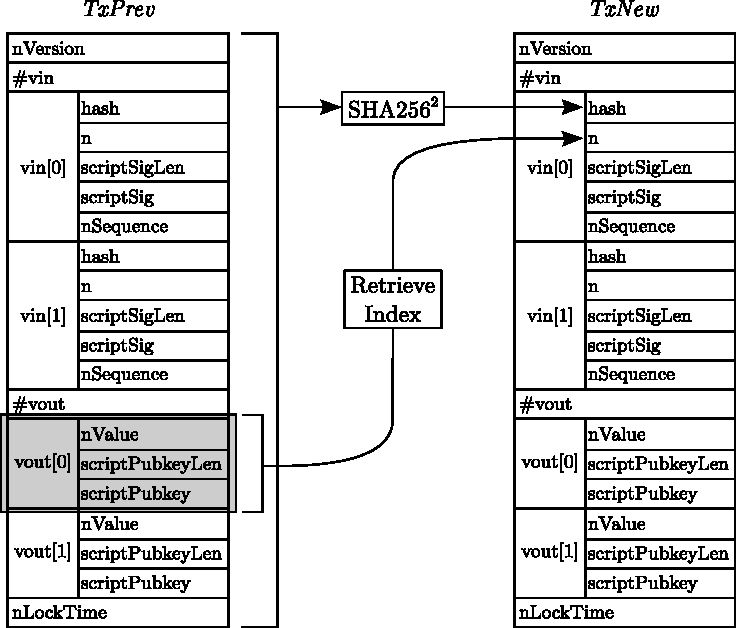
\includegraphics[scale=0.9]{images/Transaction2In2Out.pdf}
 \caption{Transaction Output Reference Computation} \label{fig:PrevOut}
\end{figure}

\item[-] \textit{scriptSigLen}~\\
This field stores the length of the signature script field \textit{scriptSig} in bytes. It is encoded as a variable length integer (see \ref{sec:DataTypes}).

\item[-] \textit{scriptSig}~\\
The signature script field contains a response script corresponding to the challenge script (see \textit{scriptPubey} field) of the referenced transaction output (\textit{hash},\textit{n}). More precisely, whilst the challenge script specifies conditions under which the transaction output can be claimed, the response script is used to prove that the transaction is allowed to claim it. More details on transaction verification can be found in Sect. \ref{sec:Script}.~\\

\item[-] \textit{nSequence}~\\
This field stores the transaction input sequence number. It was once intended for multiple signers to agree to update a transaction before including it in a block. If a signer was done updating, he marked his transaction input as final by setting the sequence number to the highest 4-byte integer value $\texttt{0xFFFFFFFF}$. More details can be found in Sect. \ref{sec:TransactionStandardness} under the Final Transaction Rule.
\end{itemize}

\subsubsection*{\#vout}
This field stores the number of elements in the output vector \textit{vout}. It is encoded as a variable length integer (see \ref{sec:DataTypes}).

\subsubsection*{vout}
The \textit{vout} field stores a vector of one or more transaction outputs. Each transaction output is composed of an amount of BTC being spent (\textit{nValue}), the length of the public key script (\textit{scriptPubkeyLen}) and the public key script (\textit{scriptPubkey}) itself.

\begin{itemize}
\item[-] \textit{nValue}~\\
The \textit{nValue} field stores the amount of BTC to be spent by the output. The amount is encoded in Satoshis, that is $10^{-8}$ BTC, allowing tiny fractions of a Bitcoin to be spent. However, note that in the reference implementation transactions with outputs less than a certain value are referred to as ``dust'' and are considered non-standard \cite{DustTransactions}. This value is currently by default 546 Satoshi and can be defined by each node manually. Dust transactions are neither relayed nor mined. More details on dust transactions can be found in \ref{sec:Calculations}.

\item[-] \textit{scriptPubkeyLen}~\\
This field stores the length of the public key script \textit{scriptPubkey} in bytes. It is encoded as a variable length integer (see \ref{sec:DataTypes}).

\item[-] \textit{scriptPubkey}~\\
The public key script field contains a challenge script for transaction verification. More precisely, whilst the challenge script specifies conditions under which the transaction output can be claimed, the response script (see \textit{scriptSig} field) is used to prove that the transaction is allowed to claim it. More details on transaction verification can be found in Sect. \ref{sec:Script}.

\end{itemize}

\subsubsection*{nLockTime}
This field stores the lock time of a transaction, i.e. a point in time past which the transaction should be included in a block. Once the lock time has been exceeded, the transaction is locked and can be included in a block. The lock time is encoded as either a timestamp in UNIX format or as a block number:
\begin{table}
\centering
	\begin{tabularx}{0.7\textwidth } {| >{\centering} m{40pt} | X |}
	\hline
	\textbf{Value} & \textbf{Description} \\ \hline\hline
	$0$ & Always locked. \\ \hline \rule{0pt}{10pt}
	$< 5*10^{8}$ & Block number at which transaction is locked. \\ \hline \rule{0pt}{10pt}
	$\geq 5*10^{8}$ & UNIX timestamp at which transaction is locked. \\ \hline
	\end{tabularx}
	\vspace{5pt}
	\caption{Lock Time Values}
	\label{tab:LockTime}
\end{table}
\vspace{-15pt}

\noindent
If all transaction inputs (see \textit{vin} field) have a final sequence number (see \mbox{\textit{nSequence}} field), then the lock time is ignored. More details can be found in Sect. \ref{sec:TransactionStandardness} under the Final Transaction Rule.


\clearpage
\subsection*{Coinbase Transactions} \label{sec:CoinbaseTransactions}
As can be seen in Table \ref{tab:TransactionCoinbase}, except for renaming the signature script field from \textit{scriptSig} to \textit{coinbase}, the data structure of the transaction remains the same. However, there are several constraints specific for a coinbase transaction. In the following the differences between a regular and a coinbase transaction will be explained.
\begin{table}[ht!]
	\begin{tabularx}{\textwidth}{ | m{30pt} | m{70pt} | >{\centering} m{60pt} | X |} \hline
		\multicolumn{2}{|l|}{\textbf{Field name}} &
		\bigcell{c}{\textbf{Type} \\ \textbf{(Size)}} &
		\textbf{Description}\\ \hline\hline
    	
    	\multicolumn{2}{|l|}{nVersion} &
    	\bigcell{c}{int \\ (4 bytes)} &
    	Transaction format version (currently 1).\\ \hline
    	
	    \multicolumn{2}{|l|}{\#vin} &
	    \bigcell{c}{VarInt \\ (1-9 bytes)} &
    	Number of transaction inputs entries in \textit{vin}. \\ \hline
    	
		\multirow{9}{30pt}{\centering vin[\,]} &
		
		hash &
		\bigcell{c}{uint256 \\ (32 bytes)} &
		Fixed double-SHA256 hash.\\ \cline{2-4}
		
		& n &
		\bigcell{c}{uint \\ (4 bytes)} &
		Fixed transaction output index. \\ \cline{2-4}

		& coinbaseLen &
		\bigcell{c}{VarInt \\ (1-9 bytes)} &
		Length of \textit{coinbase} field in bytes. \\ \cline{2-4}
				
		& coinbase &
		\bigcell{c}{CScript \\ (Variable)} &
		Encodes the block height and arbitrary data. \\ \cline{2-4}
		
		& nSequence &
		\bigcell{c}{uint \\ (4 bytes)} &
		Transaction input sequence number.\\ \hline
    	
    	\multicolumn{2}{|l|}{\#vout} &
	    \bigcell{c}{VarInt \\ (1-9 bytes)} &
    	Number of transaction output entries in \textit{vout}. \\ \hline
    	
		\multirow{5}{30pt}{\centering vout[\,]} &
		
		nValue &
		\bigcell{c}{int64\_t \\ (8 bytes)} &
		Amount of $10^{-8}$ BTC. \\ \cline{2-4}
		
		& scriptPubkeyLen &
		\bigcell{c}{VarInt \\ (1-9 bytes)} &
		Length of \textit{scriptPubkey} field in bytes. \\ \cline{2-4}

		& scriptPubkey &
		\bigcell{c}{CScript \\ (Variable)} &
		Script specifying conditions under which the transaction output can be claimed. \\ \hline
    	
    	\multicolumn{2}{|l|}{nLockTime} &
    	\bigcell{c}{unsigned int \\ (4 bytes)} &
    	Timestamp until which transactions can be replaced before block inclusion.\\ \hline
	
	\end{tabularx}
	\vspace{5pt}
	\caption{Transaction Structure Description (Coinbase Transactions)}
	\label{tab:TransactionCoinbase}
\end{table}
\vspace{-20pt}

\subsubsection*{\#vin}
The number of inputs stored in the input vector \textit{vin} is always 1.

\subsubsection*{vin}
The \textit{vin} field stores a vector of precisely one transaction input. The input is composed of a fixed transaction output reference (\textit{hash},\textit{n}), the length of the coinbase field in bytes (\textit{coinbaseLen}), the coinbase field (\textit{coinbase}) itself and a transaction sequence number (\textit{nSequence}).

\begin{itemize}
\item[-] (\textit{hash},\textit{n})~\\
In a coinbase transaction new coins are introduced into the system and therefore no previous transaction output is referenced. The (\textit{hash},\textit{n}) tuple stores the following constant values:
\begin{equation}
\begin{split}
hash &=\ 0 \\
n &=\ 2^{32}-1
\end{split}
\end{equation}

\item[-] \textit{coinbaseLen}~\\
This field stores the length of the coinbase field \textit{coinbase} in bytes. It is in the range of 2-100 bytes and is encoded as a variable length integer (see \ref{sec:DataTypes}).

\item[-] \textit{coinbase}~\\
The coinbase field, also referred to as the coinbase script, stores the block height, i.e. the block number within the blockchain, and arbitrary data.~\\

\vspace{-10pt}
\begin{table}
	\centering
	\begin{tabularx}{0.888\textwidth}{| m{70pt} | >{\centering} m{80pt} | X |}
	\hline
	\textbf{Field name} &
	\textbf{Size (bytes)} &
	\textbf{Description} \\ \hline \hline
	
	blockHeightLen &
	1 &
	Length of \textit{blockHeight} field in bytes. \\ \hline
	
	blockHeight &
	\textit{blockHeightLen} &
	Block height encoding. \\ \hline
	
	arbitraryData &
	$\textit{coinbaseLen} - (\textit{blockHeightLen} + 1)$ &
	Arbitrary data field. \\ \hline
	
	\end{tabularx}
	\vspace{5pt}
	\caption{Coinbase Field Encoding}
	\label{tab:CoinbaseFieldEncoding}
\end{table}
\vspace{-20pt}

As of BIP0034 \cite{BIP0034}, the beginning of the coinbase field is reserved for the block height. It is encoded in serialized Script format, i.e. the first byte specifies the size of the block height in bytes, followed by the block height itself in little-endian notation. The remaining bytes can be chosen arbitrarily and serve as a degree-of-freedom for the proof-of-work puzzle (see Sect. \ref{sec:Mining}).
\end{itemize} 


\subsubsection*{vout}
The transaction output vector is constrained by the maximal amount of Bitcoins that is allowed to be transacted. More precisely, there are certain rules how the \textit{nValue} field is to be calculated.

\begin{itemize}
\item[-] \textit{nValue}~\\
In a coinbase transaction the miner is allowed to claim the current mining subsidy, as well as transaction fees for all included transactions, as a reward for solving the proof-of-work puzzle. The subsidy for finding a valid block is currently 25 BTC and is halved every 210000 blocks. The transaction fee, on the other hand, is computed for each transaction as the difference between the sum of input values and the sum of output values.
\end{itemize}


\subsection{Transaction Standardness} \label{sec:TransactionStandardness}
Transaction standardness is defined as a set of requirements that is enforced upon a transaction by any node utilizing the reference client for transaction processing. Transactions that do not meet all the requirements are considered non-standard and will be neither relayed nor mined. Note that these rules are not enforced upon transactions of an already mined block. It is thus allowed to mine and include non-standard transactions in blocks. The transaction standardness rules are as follows.

\subsubsection*{Transaction Size}
A single transaction may not exceed 10000 bytes in size.

\subsubsection*{Transaction Version}
The transaction format version is currently 1.

\subsubsection*{Final Transaction Rule} \label{sec:FinalTransaction}
It is said that a transaction is final if it satisfies at least one of the following conditions:

\begin{enumerate}[label=\arabic*), leftmargin=1cm]
\item The transaction lock time (see \textit{nLockTime} field) is set to locked or has been exceeded.
\item All transaction inputs are final (see \textit{nSequence} field).
\end{enumerate}

\noindent
This rule is associated with an obsolete mechanism called transaction replacement. It allowed to replace certain parts of a transaction, e.g. transaction inputs, until either all transaction inputs were finalized or the transaction lock time has passed. Note, however, that the transaction replacement functionality has been completely removed from the reference implementation to reduce the complexity of the protocol and although the transaction lock time functionality is still in place, it is considered non-standard.

\subsubsection*{Transaction Input Rules}
For each transaction input the following requirements must be satisfied by each signature script field:

\begin{enumerate}[label=\arabic*), leftmargin=1cm]
\item \textit{Signature Script Size}~\\The size may not exceed 500 bytes. Note that this limitation will change to 1650 bytes in the next major release of the reference client.
\item \textit{Push Only}~\\Only a restricted set of data push operations is allowed. To be specific, only opcodes\footnote{See \textit{https://en.bitcoin.it/wiki/Script} for complete reference.} in the range \texttt{0x00}-\texttt{0x60} are permitted.
\item \textit{Canonical Pushes}~\\The scripting language allows to push data on the stack in different ways. This rule enforces that only data pushes intended for a particular data size are allowed.
\end{enumerate}

\subsubsection*{Transaction Output Rules}
For each transaction output the following requirements must be satisfied:

\begin{enumerate}[label=\arabic*), leftmargin=1cm]
\item \textit{Standard Transaction Type}~\\The public key script field (\textit{scriptPubkey}) must encode a standard transaction type (see Sect. \ref{sec:StandardTxTypes}).
\item \textit{Non-Dust Transaction}~\\The transaction is not allowed to be ``dust''. A transaction is called ``dust'' if it contains an output that spends more than 1/3rd's in transaction fees (see \ref{sec:Calculations} for calculation of the fee).
\end{enumerate}

\subsubsection*{Nulldata Transaction Count}
At most one transaction output of Nulldata transaction type (see Sect. \ref{sec:StandardTxTypes}) per transaction is permitted.

\clearpage
\section{Bitcoin ownership} \label{sec:BitcoinOwnership}

\subsection{General} \label{sec:OwnershipGeneral}
Bitcoin utilizes two cryptographic primitives to realize a secure and decentralized transaction authorization system. Firstly, it employs asymmetric cryptography for (i) identification and (ii) authentication of recipients, as well as to (iii) ensure integrity of regular transactions. More precisely, the public key of a public/private keypair is used to identify a particular recipient, whereas the private key is used to create a signature for both transaction authentication and integrity.~\\

\noindent
Secondly, the proof of work protocol is used to (i) regulate coin supply, (ii) reward miners for transaction processing and (iii) ensure block integrity. In the mining process all regular transactions of users and a special coinbase transaction created by the miner are processed by solving the proof of work problem. It is important to note that while the authenticity and integrity of regular transactions is ensured by the previously discussed signature scheme, the integrity of coinbase transactions is assured by the proof of work puzzle. In the following the exact application of these primitives will be described with the help of Fig. \ref{fig:TransactionChain}.

\vspace{-5pt}
\begin{figure}[htbp]
\centering
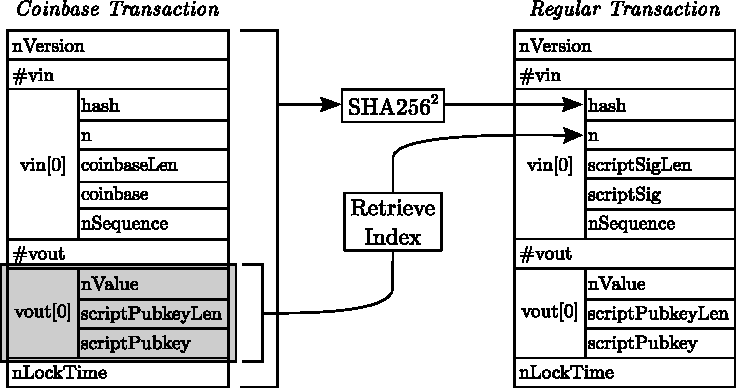
\includegraphics[scale=1]{Images/Ownership.pdf}

\caption{Bitcoin Transaction Chain}
\label{fig:TransactionChain}
\end{figure}
\vspace{-10pt}

\noindent
To begin with, Bitcoins are introduced into the system with coinbase transactions (see Sect. \ref{sec:CoinbaseTransactions}). In it the miner specifies one or more transaction outputs (\textit{vout}), defining the amounts and destinations to which the freshly created coins are to be transferred. He identifies each destination by including a public key or a derived form of it in the public key script field (\textit{scriptPubkey}). As discussed above, the integrity of the coinbase transaction is ensured by the computational hardness of the proof of work problem.~\\

\noindent
Next, when the miner intends to spend his reward, he creates a regular transaction, references it to the specific output of the coinbase transaction and provides a signature in the signature script field (\textit{scriptSig}). Since the signature is computed over the complete transactions (see Sect. \ref{sec:Signatures}), control of the private key corresponding to the referenced public key is proven and integrity of the transaction is guaranteed. This chain is continued indefinitely and logged publicly in the blockchain to keep track of all Bitcoins within the system at all times.


\subsection{Script} \label{sec:Script}
Script is a stack-based, Turing-incomplete language designed specifically for the Bitcoin protocol. A script is essentially a set of instructions\footnote{See \textit{https://en.bitcoin.it/wiki/Script} for complete reference.} that are processed left to right. Script is used to encode two components - a challenge script and a response script:

\begin{itemize}
\item[-] A challenge script (see \textit{scriptPubkey} field) is part of a transaction output and specifies under which conditions it can be claimed.
\item[-] A response script (see \textit{scriptSig} field) is part of a transaction input and is used to prove that the referenced transaction output can be rightfully claimed.
\end{itemize}

\noindent
For a given transaction, each transaction input is verified by first evaluating \textit{scriptSig}, then copying the resulting stack and finally evaluating \textit{scriptPubkey} of the referenced transaction output. If during the evaluation no failure is triggered and the final top stack element yields true, then the ownership has been successfully verified.~\\

\noindent
Although Script is very comprehensive and allows one to construct intricate conditions under which coins can be claimed, much of its functionality is currently disabled in the reference implementation and only a restricted set of standard script templates is accepted. These are \textit{Pay-to-Pubkey} (P2PK), \textit{Pay-to-PubkeyHash} (P2PKH), \textit{Pay-to-ScriptHash} (P2SH), \textit{Multisig} and \textit{Nulldata}. In the next section, the structure of these standard transaction types will be discussed.~\\


\clearpage
\enlargethispage{2\baselineskip}
\subsection{Standard Transaction Types} \label{sec:StandardTxTypes}
\vspace{6pt}

\subsubsection{Pay-to-Pubkey (P2PK)} \label{sec:P2PK}
The structure of the challenge and response scripts of a Pay-to-Pubkey transaction are depicted below in Fig. \ref{fig:P2PubStructure}. Note that operations in a script are written as \texttt{OP\_X}, where \texttt{OP} stands for operation and \texttt{X} is an abbreviation of the operation's function. For example, in Fig. \ref{fig:P2PubStructure} \texttt{CHECKSIG} stands for signature verification.

\vspace{-10pt}
\begin{figure}[htbp]

\begin{Verbatim}[fontsize==\relsize{-4}, frame=single]  
scriptPubkey: <pubkey> OP_CHECKSIG
scriptSig:    <signature>
\end{Verbatim}

\vspace{-15pt}
\caption{Pay-to-Pubkey Structure}
\label{fig:P2PubStructure}
\end{figure}
\vspace{-10pt}

\noindent
In a Pay-to-Pubkey transaction the sender transfers Bitcoins directly to the owner of a public key. He specifies in the challenge script the public key (\textit{pubkey}) and one requirement that the claimant has to prove:
\begin{enumerate}[label=\arabic*), leftmargin=1cm]
\item Knowledge of the private key corresponding to the public key.
\end{enumerate}

\noindent
To do so, the claimant creates a response script containing only a signature. The scripts are then evaluated as depicted in Table \ref{tab:P2Pub1} and \ref{tab:P2Pub2}. The signature and the public key are pushed onto the stack and evaluated. Note that the signature is computed as described in Sect. \ref{sec:Signatures}.


\begin{table}
\begin{minipage}{\textwidth}

\centering
\begin{tabular}{| m{95pt} | m{145pt} | m{100pt} |} \hline
\textbf{Stack} & \textbf{Remaining Script} & \textbf{Description} \\ \hline \hline

\vspace{8pt}
\begin{BVerbatim}[fontsize==\relsize{-4}]
Empty
\end{BVerbatim} 
\vspace{4pt}
&
\vspace{8pt}
\begin{BVerbatim}[fontsize==\relsize{-4}]
<signature>
\end{BVerbatim} 
\vspace{4pt}
&
The signature is pushed on the stack.\\ \hline

\vspace{8pt}
\begin{BVerbatim}[fontsize==\relsize{-4}]
<signature>
\end{BVerbatim} 
\vspace{4pt}
&
\vspace{8pt}
\begin{BVerbatim}[fontsize==\relsize{-4}]
Empty
\end{BVerbatim} 
\vspace{4pt}
&
Final state after evaluating \textit{scriptSig}. \\ \hline

\end{tabular}
\vspace{5pt}
\caption{Pay-to-Pubkey \textit{scriptSig} Execution}
\label{tab:P2Pub1}

\vspace{15pt}

\begin{tabular}{| m{95pt} | m{145pt} | m{100pt} |}
\hline
\textbf{Stack} & \textbf{Remaining Script} & \textbf{Description} \\ \hline \hline

\vspace{8pt}
\begin{BVerbatim}[fontsize==\relsize{-4}]
<signature>
\end{BVerbatim}
\vspace{4pt}
&
\vspace{8pt}
\begin{BVerbatim}[fontsize==\relsize{-4}]
<pubkey> OP_CHECKSIG
\end{BVerbatim} 
\vspace{4pt}
&
State after copying the stack of the signature script evaluation. The public key is pushed on the stack.\\ \hline	

\vspace{8pt}
\begin{BVerbatim}[fontsize==\relsize{-4}]
<pubkey>
<signature>
\end{BVerbatim}
\vspace{4pt}
&
\vspace{8pt}
\begin{BVerbatim}[fontsize==\relsize{-4}]
OP_CHECKSIG
\end{BVerbatim} 
\vspace{4pt}
&
The signature is verified for the top two stack elements and the result is pushed on the stack.\\ \hline	


\vspace{8pt}
\begin{BVerbatim}[fontsize==\relsize{-4}]
True
\end{BVerbatim}
\vspace{4pt}
&
\vspace{8pt}
\begin{BVerbatim}[fontsize==\relsize{-4}]
Empty
\end{BVerbatim} 
\vspace{4pt}
&
Final state after evaluating \textit{scriptPubkey}. \\ \hline

\end{tabular}
\vspace{5pt}
\caption{Pay-to-Pubkey \textit{scriptPubkey} Execution}
\label{tab:P2Pub2}

\end{minipage}
\end{table}

\clearpage
\subsubsection{Pay-to-PubkeyHash (P2PKH)} \label{sec:P2PKH}
The structure of the challenge and response scripts of a Pay-to-PubkeyHash transaction can be seen below in Fig. \ref{fig:P2PubHashStructure}.

\vspace{-10pt}
\begin{figure}[ht!]

\begin{Verbatim}[fontsize==\relsize{-4}, frame=single]  
scriptPubkey: OP_DUP OP_HASH160 <pubkeyHash> OP_EQUALVERIFY OP_CHECKSIG
scriptSig:    <signature> <pubkey>	
\end{Verbatim}

\vspace{-15pt}
\caption{Pay-to-PubkeyHash Structure}
\label{fig:P2PubHashStructure}
\end{figure}
\vspace{-10pt}

\noindent
In a Pay-to-PubkeyHash transaction the sender transfers Bitcoins to the owner of a P2PKH address (see Sect. \ref{sec:Address-P2PKH}). He specifies in the challenge script the public key hash (\textit{pubkeyHash}) of the Bitcoin address (depicted in Fig. \ref{fig:BitcoinAddress-P2PKH}) and two requirements that the claimant has to prove:

\begin{enumerate}[label=\arabic*), leftmargin=1cm]
\item Knowledge of the public key corresponding to \textit{pubkeyHash}.
\item Knowledge of the private key corresponding to the public key.
\end{enumerate}

\noindent
To do so, the claimant creates a response script containing a signature and a public key. The scripts are then evaluated as depicted in Table \ref{tab:P2PubHash1} and \ref{tab:P2PubHash2}. First, it is verified if the public key (\textit{pubkey}) corresponds to the public key hash (\textit{pubkeyHash}) and then whether the signature is valid. The signature is computed as described in Sect. \ref{sec:Signatures}.~\\


\begin{table}[!ht]
  
\begin{minipage}{\textwidth}

\centering
\begin{tabular}{| m{95pt} | m{145pt} | m{100pt} |}
\hline
\textbf{Stack} & \textbf{Remaining Script} & \textbf{Description} \\ \hline \hline

\vspace{8pt}
\begin{BVerbatim}[fontsize==\relsize{-4}]
Empty
\end{BVerbatim} 
\vspace{4pt}
&
\vspace{8pt}
\begin{BVerbatim}[fontsize==\relsize{-4}]
<signature> <pubkey>
\end{BVerbatim} 
\vspace{4pt}
&
The signature and the public key are pushed on the stack. \\ \hline


\vspace{8pt}
\begin{BVerbatim}[fontsize==\relsize{-4}]
<pubkey>
<signature>
\end{BVerbatim} 
\vspace{4pt}
&
\vspace{8pt}
\begin{BVerbatim}[fontsize==\relsize{-4}]
Empty
\end{BVerbatim} 
\vspace{4pt}
&
Final state after evaluating \textit{scriptSig}. \\ \hline

\end{tabular}
\vspace{5pt}
\caption{Pay-to-PubkeyHash \textit{scriptSig} Execution}
\label{tab:P2PubHash1}

\vspace{15pt}

\centering
\begin{tabular}{| m{95pt} | m{145pt} | m{100pt} |}
\hline
\textbf{Stack} & \textbf{Remaining Script} & \textbf{Description} \\ \hline \hline

\vspace{8pt}
\begin{BVerbatim}[fontsize==\relsize{-4}]
<pubkey>
<signature>
\end{BVerbatim}
\vspace{4pt}
&
\vspace{8pt}
\begin{BVerbatim}[fontsize==\relsize{-4}]
OP_DUP OP_HASH160 <pubkeyHash>
OP_EQUALVERIFY OP_CHECKSIG
\end{BVerbatim} 
\vspace{4pt}
&
State after copying the stack of the signature script evaluation. The top stack element is duplicated.\\ \hline


\vspace{8pt}
\begin{BVerbatim}[fontsize==\relsize{-4}]
<pubkey>
<pubkey>
<signature>
\end{BVerbatim}
\vspace{4pt}
&
\vspace{8pt}
\begin{BVerbatim}[fontsize==\relsize{-4}]
OP_HASH160 <pubkeyHash>
OP_EQUALVERIFY OP_CHECKSIG
\end{BVerbatim} 
\vspace{4pt}
&
The top stack element is first hashed with SHA256 and then with RIPEMD160.\\ \hline


\vspace{8pt}
\begin{BVerbatim}[fontsize==\relsize{-4}]
<pubkeyHashNew>
<pubkey>
<signature>
\end{BVerbatim}
\vspace{4pt}
&
\vspace{8pt}
\begin{BVerbatim}[fontsize==\relsize{-4}]
<pubkeyHash> OP_EQUALVERIFY
OP_CHECKSIG
\end{BVerbatim} 
\vspace{4pt}
&
The public key hash is pushed on the stack.\\ \hline

	
\vspace{8pt}
\begin{BVerbatim}[fontsize==\relsize{-4}]
<pubkeyHash>
<pubkeyHashNew>
<pubkey> 
<signature>
\end{BVerbatim}
\vspace{4pt}
&
\vspace{8pt}
\begin{BVerbatim}[fontsize==\relsize{-4}]
OP_EQUALVERIFY OP_CHECKSIG
\end{BVerbatim} 
\vspace{4pt}
&
Equality of the top two stack elements is checked. If it evaluates to true then execution is continued. Otherwise it fails.\\ \hline


\vspace{8pt}
\begin{BVerbatim}[fontsize==\relsize{-4}]
<pubkey>
<signature>
\end{BVerbatim}
\vspace{4pt}
&
\vspace{8pt}
\begin{BVerbatim}[fontsize==\relsize{-4}]
OP_CHECKSIG
\end{BVerbatim} 
\vspace{4pt}
&
The signature is verified for the top two stack elements.\\ \hline


\vspace{8pt}
\begin{BVerbatim}[fontsize==\relsize{-4}]
True
\end{BVerbatim}
\vspace{4pt}
&
\vspace{8pt}
\begin{BVerbatim}[fontsize==\relsize{-4}]
Empty
\end{BVerbatim} 
\vspace{4pt}
&
Final state after evaluating \textit{scriptPubkey}.\\ \hline

\end{tabular}
\vspace{5pt}
\caption{Pay-to-PubkeyHash \textit{scriptPubkey} Execution}
\label{tab:P2PubHash2}

\end{minipage}
\end{table}

\clearpage
\subsubsection{Pay-to-ScriptHash (P2SH)} \label{sec:P2SH}
The structure of the challenge and response scripts of a Pay-to-ScriptHash transaction is depicted below in Fig. \ref{fig:P2ScriptHashStructure}.

\vspace{-10pt}
\begin{figure}[htbp]

\begin{Verbatim}[fontsize==\relsize{-4}, frame=single]  
scriptPubkey: OP_HASH160 <scriptHash> OP_EQUAL
scriptSig:    <signatures> {serializedScript}
\end{Verbatim}

\vspace{-15pt}
\caption{Pay-to-ScriptHash Structure}
\label{fig:P2ScriptHashStructure}
\end{figure}
\vspace{-10pt}

\noindent
In a Pay-to-ScriptHash transaction the sender transfers Bitcoins to the owner of a P2SH Bitcoin address (see Sect. \ref{sec:Address-P2SH}). He specifies in the challenge script the serialized script hash (\textit{scriptHash}) of the Bitcoin address (depicted in Fig. \ref{fig:BitcoinAddress-P2SH}) and one requirement that the claimant has to prove:

\begin{enumerate}[label=\arabic*), leftmargin=1cm]
\item Knowledge of the redemption script \textit{serializedScript} corresponding to\\ \textit{scriptHash}.
\end{enumerate}

\noindent
To do so, the claimant creates a response script containing one or more signatures and the serialized redemption script \textit{serializedScript}. Note that unlike in any other standard transaction type the responsibility of supplying the conditions for redeeming the transaction is shifted from the sender to the redeemer. The redeemer may specify any conditions in the redemption script \textit{serializedScript} conforming to standard transaction types. For example, he may define a standard Pay-to-Pubkey transaction as a Pay-to-ScriptHash transaction as follows:

\vspace{-10pt}
\begin{figure}[htbp]

\begin{Verbatim}[fontsize==\relsize{-4}, frame=single]  
scriptPubkey: OP_HASH160 <scriptHash> OP_EQUAL
scriptSig:    <signatures> {<pubkey> OP_CHECKSIG}
\end{Verbatim}

\vspace{-15pt}
\caption{P2SH Pay-to-PublicKey Structure}
\label{fig:P2ScriptHashStructure-P2PK}
\end{figure}
\vspace{-10pt}

\noindent
Due to the nested nature of this transaction type, the script evaluation requires an additional validation step. First, it is verified whether the redemption script (\textit{serializedScript}) is consistent with the redemption script hash (\textit{scriptHash}) and then the transaction is evaluated using the redemption script as \textit{scriptPubkey}. The evaluation is depicted in Table \ref{tab:P2ScriptHash1}, \ref{tab:P2ScriptHash2} and \ref{tab:P2ScriptHash3}.

\clearpage

\begin{table}[!ht]  
\begin{minipage}{\textwidth}

\centering
\begin{tabular}{| m{105pt} | m{135pt} | m{100pt} |}
\hline
\textbf{Stack} & \textbf{Remaining Script} & \textbf{Description} \\ \hline \hline

\vspace{8pt}
\begin{BVerbatim}[fontsize==\relsize{-4}]
Empty
\end{BVerbatim} 
\vspace{4pt}
&
\vspace{8pt}
\begin{BVerbatim}[fontsize==\relsize{-4}]
<signature>
{<pubkey> OP_CHECKSIG}
\end{BVerbatim} 
\vspace{4pt}
&
The signature and the redemption script are pushed on the stack. \\ \hline


\vspace{8pt}
\begin{BVerbatim}[fontsize==\relsize{-4}]
{<pubkey> OP_CHECKSIG}
<signature>
\end{BVerbatim} 
\vspace{4pt}
&
\vspace{8pt}
\begin{BVerbatim}[fontsize==\relsize{-4}]
Empty
\end{BVerbatim} 
\vspace{4pt}
&
Final state after evaluating \textit{scriptSig}. \\ \hline

\end{tabular}
\vspace{5pt}
\caption{Pay-to-ScriptHash \textit{scriptSig} Execution}
\label{tab:P2ScriptHash1}


\vspace{15pt}


\centering
\begin{tabular}{| m{105pt} | m{135pt} | m{100pt} |}
\hline
\textbf{Stack} & \textbf{Remaining Script} & \textbf{Description} \\ \hline \hline

\vspace{8pt}
\begin{BVerbatim}[fontsize==\relsize{-4}]
{<pubkey> OP_CHECKSIG}
<signature>
\end{BVerbatim} 
\vspace{4pt}
&
\vspace{8pt}
\begin{BVerbatim}[fontsize==\relsize{-4}]
OP_HASH160 <scriptHash>
OP_EQUAL
\end{BVerbatim} 
\vspace{4pt}
&
State after copying the stack of the signature script evaluation. The top stack element is first hashed with SHA256 and then with RIPEMD160.\\ \hline


\vspace{8pt}
\begin{BVerbatim}[fontsize==\relsize{-4}]
<scriptHashNew>
<signature>
\end{BVerbatim} 
\vspace{4pt}
&
\vspace{8pt}
\begin{BVerbatim}[fontsize==\relsize{-4}]
<scriptHash> OP_EQUAL
\end{BVerbatim} 
\vspace{4pt}
&
The redemption script hash is pushed on the stack.\\ \hline


\vspace{8pt}
\begin{BVerbatim}[fontsize==\relsize{-4}]
<scriptHash>
<scriptHashNew>
<signature>
\end{BVerbatim} 
\vspace{4pt}
&
\vspace{8pt}
\begin{BVerbatim}[fontsize==\relsize{-4}]
OP_EQUAL
\end{BVerbatim} 
\vspace{4pt}
&
Equality of the top two stack elements is checked. The result of the evaluation is pushed on the stack.\\ \hline


\vspace{8pt}
\begin{BVerbatim}[fontsize==\relsize{-4}]
True
<signature>
\end{BVerbatim} 
\vspace{4pt}
&
\vspace{8pt}
\begin{BVerbatim}[fontsize==\relsize{-4}]
Empty
\end{BVerbatim} 
\vspace{4pt}
&
Final state after evaluating \textit{scriptPubkey}.\\ \hline

\end{tabular}
\vspace{5pt}
\caption{Pay-to-ScriptHash \textit{scriptPubkey} Execution}
\label{tab:P2ScriptHash2}
\end{minipage}
\end{table}

\vspace{-10pt}

\noindent
For the additional validation step the stack after \textit{scriptSig} execution (see Table \ref{tab:P2ScriptHash1}) is copied, the top stack element is popped and used as the script. The state now resembles the beginning of a standard Pay-to-Pubkey transaction evaluation (see Table \ref{tab:P2Pub2}).

\begin{table}[!h]  
	
	\centering
	\begin{tabular}{| m{105pt} | m{135pt} | m{100pt} |}
		\hline
		\textbf{Stack} & \textbf{Remaining Script} & \textbf{Description} \\ \hline \hline
		
		\vspace{8pt}
\begin{BVerbatim}[fontsize==\relsize{-4}]
<signature>
\end{BVerbatim} 
		\vspace{4pt}
		&
		\vspace{8pt}
\begin{BVerbatim}[fontsize==\relsize{-4}]
<pubkey> OP_CHECKSIG
\end{BVerbatim} 
		\vspace{4pt}
		&
		Initial state of supplementary validation step.\\ \hline
		
		\dots & \dots & \dots \\ \hline
	\end{tabular}
	
\vspace{5pt}
\caption{Pay-to-ScriptHash Supplementary Validation}
\label{tab:P2ScriptHash3}
\end{table}


\clearpage
\subsubsection{Multisig} \label{sec:Multisig}
The structure of the challenge and response scripts of a Multisig transaction is depicted below in Fig. \ref{fig:P2Multisig}.

\vspace{-10pt}
\begin{figure}[htbp]

\begin{Verbatim}[fontsize==\relsize{-4}, frame=single]  
scriptPubkey: m <pubkey 1> ... <pubkey n> n OP_CHECKMULTISIG
scriptSig:    OP_0 <signature 1> ... <signature m>
\end{Verbatim}

\vspace{-15pt}
\caption{Multisig Structure}
\label{fig:P2Multisig}
\end{figure}
\vspace{-10pt}

\noindent
In a Multisig transaction the sender transfers Bitcoins to the owner of \textit{m}-of-\textit{n} public keys. He specifies in the challenge script \textit{n} public keys (\textit{pubkey 1..n}) and a requirement that the claimant has to prove:

\begin{enumerate}[label=\arabic*), leftmargin=1cm]
\item Knowledge of at least \textit{m} private keys corresponding to the public keys.
\end{enumerate}

\noindent
To do so, the claimant creates a response script containing at least \textit{m} signatures in the same order of appearance as the public keys. Note that due to an off-by-one error {\tt OP\_CHECKMULTISIG} pops one too many elements off the stack and it is therefore required to prepend the response script with a zero data push {\tt OP\_0}. The script is then evaluated as depicted in Table \ref{tab:P2Multisig1} and \ref{tab:P2Multisig2}. First, the signatures are pushed on the stack, followed by the number of required signatures \textit{m}, the public keys and the number of public keys \textit{n}.~\\

\noindent
The bounds for a standard Multisig transaction are $1 \leq m \leq n \leq 3$, whereas for a P2SH Multisig transaction they are variable. The upper bound for a P2SH Multisig transaction is restricted by both the allowed size of the signature script \textit{scriptSig} (500 bytes) and the allowed size of the serialized script \textit{serializedScript} (520 bytes). It is therefore possible to create e.g. a 1-of-12 P2SH Multisig transaction with compressed public keys or a 4-of-5 P2SH Multisig transaction with compressed public keys. Note that the maximum size of the signature script field (\textit{scriptSig}) will be increased in the next major release to 1650 bytes, thus allowing even bigger P2SH Multisig transactions.

\begin{table}[!ht]  
\begin{minipage}{\textwidth}

\centering
\begin{tabular}{| m{95pt} | m{145pt} | m{100pt} |}

\hline
\textbf{Stack} & \textbf{Remaining Script} & \textbf{Description} \\ \hline \hline

\vspace{8pt}
\begin{BVerbatim}[fontsize==\relsize{-4}]
Empty
\end{BVerbatim} 
\vspace{4pt}
&
\vspace{8pt}
\begin{BVerbatim}[fontsize==\relsize{-4}]
OP_0 <signature 1> ...
<signature m>
\end{BVerbatim} 
\vspace{4pt}
&
The signatures are pushed on the stack.\\ \hline

\vspace{8pt}
\begin{BVerbatim}[fontsize==\relsize{-4}]
<signature m>
...
<signature 1>
OP_0
\end{BVerbatim} 
\vspace{4pt}
&
\vspace{8pt}
\begin{BVerbatim}[fontsize==\relsize{-4}]
Empty
\end{BVerbatim} 
\vspace{4pt}
&
Final state after evaluating \textit{scriptSig}. \\ \hline

\end{tabular}
\vspace{5pt}
\caption{Multisig \textit{scriptSig} Execution}
\label{tab:P2Multisig1}


\vspace{15pt}


\begin{tabular}{| m{95pt} | m{145pt} | m{100pt} |}
\hline
\textbf{Stack} & \textbf{Remaining Script} & \textbf{Description} \\ \hline \hline

\vspace{8pt}
\begin{BVerbatim}[fontsize==\relsize{-4}]
<signature m>
...
<signature 1>
OP_0
\end{BVerbatim}
\vspace{4pt}
&
\vspace{8pt}
\begin{BVerbatim}[fontsize==\relsize{-4}]
m <pubkey 1> ... <pubkey n> n
OP_CHECKMULTISIG
\end{BVerbatim} 
\vspace{4pt}
&
State after copying the stack of the signature script evaluation. The public keys are pushed on the stack.\\ \hline	

\vspace{8pt}
\begin{BVerbatim}[fontsize==\relsize{-4}]
n
<pubkey n>
...
<pubkey 1>
m
<signature m>
...
<signature 1>
OP_0
\end{BVerbatim}
\vspace{4pt}
&
\vspace{8pt}
\begin{BVerbatim}[fontsize==\relsize{-4}]
OP_CHECKMULTISIG
\end{BVerbatim} 
\vspace{4pt}
&
The signatures are verified in order of appearance and the result is pushed on the stack.\\ \hline	


\vspace{8pt}
\begin{BVerbatim}[fontsize==\relsize{-4}]
True
\end{BVerbatim}
\vspace{4pt}
&
\vspace{8pt}
\begin{BVerbatim}[fontsize==\relsize{-4}]
Empty
\end{BVerbatim} 
\vspace{4pt}
&
Final state after evaluating \textit{scriptPubkey}.\\ \hline

\end{tabular}
\vspace{5pt}
\caption{Multisig \textit{scriptPubkey} Execution}
\label{tab:P2Multisig2}

\end{minipage}
\end{table}

\clearpage
\subsubsection{Nulldata}
The structure of the challenge and response scripts of a Nulldata transaction is depicted below in Fig. \ref{fig:Nulldata}.

\vspace{-10pt}
\begin{figure}[htbp]

\begin{Verbatim}[fontsize==\relsize{-4}, frame=single]  
scriptPubkey: OP_RETURN [SMALLDATA]
scriptSig:    
\end{Verbatim}

\vspace{-15pt}
\caption{Nulldata Structure}
\label{fig:Nulldata}
\end{figure}
\vspace{-10pt}

\noindent
Unlike all other standard transaction types, a Nulldata transaction does not specify in the challenge script any recipients and does not have a corresponding response script. Another characteristic of it is that it does not adhere to the dust transaction rule (see \ref{sec:Formulas}) and therefore the transaction output value can be set to zero.~\\

\noindent
The purpose of Nulldata transactions is to allow inclusion of arbitrary data in transactions in a controlled fashion. For this reason these transactions possess an optional field in which up to 40 bytes of data can be stored. Note, however, that in order to prevent blockchain flooding only one output of this type is permitted in a transaction.


\clearpage
\subsection{Bitcoin Addresses} \label{sec:BitcoinAddresses}
A Bitcoin address is a unique, 27-34 alphanumeric characters long identifier that can be used as a destination for Bitcoin payments. There are currently two different types of Bitcoin addresses in existence, \emph{Pay-to-PubkeyHash} and \emph{Pay-to-ScriptHash}, which are used in conjunction with their corresponding transaction type. In the following both will be described in detail.

\subsubsection{Pay-to-PubkeyHash Address} \label{sec:Address-P2PKH}
Essentially, a Pay-to-PubkeyHash address is a hash of the public key portion of the public-private ECDSA keypair with a built-in checksum. Schematics of how it is calculated can be seen in Fig. \ref{fig:BitcoinAddress-P2PKH}.~\\

\noindent
First, the EC public key is hashed using SHA256 and RIPEMD160. The resulting structure is referred to as \textit{pubkeyHash}. Next, a constant version byte is prepended to \textit{pubkeyHash}. A checksum is built over it by applying a double-SHA256 hash and truncating the result to the first 4 bytes. The checksum is then appended. Finally, the result is converted into a human-readable string using Base58 encoding \cite{Base58}. The final result is a \emph{P2PKH address}.

\begin{figure}[htbp]

\centering
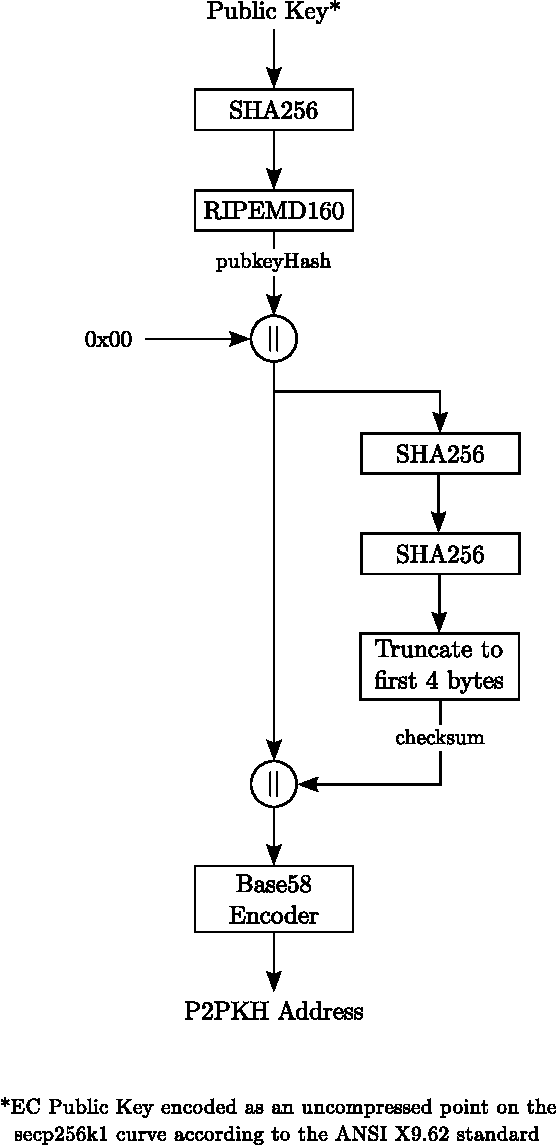
\includegraphics[scale=0.9]{Images/BitcoinAddress-P2PKH.pdf}

\vspace{10pt}
\caption{P2PKH Address Computation}
\label{fig:BitcoinAddress-P2PKH}
\end{figure}
\vspace{-10pt}


\subsubsection{Pay-to-ScriptHash Address} \label{sec:Address-P2SH}
A Pay-to-ScriptHash address on the other hand, is a hash of the redemption script \textit{serializedScript}, with a built-in checksum. Schematics of how it is calculated can be seen in Fig. \ref{fig:BitcoinAddress-P2SH}.~\\

\noindent
First, the redemption script is hashed using SHA256 and RIPEMD160. The resulting structure is referred to as \textit{scriptHash}. Next, a constant version byte is prepended to \textit{scriptHash}. A checksum is built over it by applying a double-SHA256 hash and truncating the result to the first 4 bytes. The checksum is then appended. Finally, the result is converted into a human-readable string using Base58 encoding \cite{Base58}. The final result is a \emph{P2SH address}.

\begin{figure}[htbp]

\centering
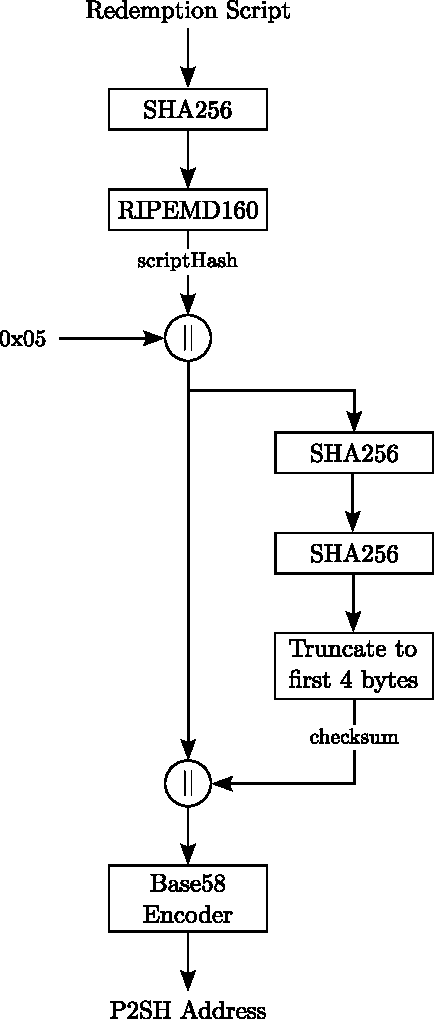
\includegraphics[scale=0.9]{Images/BitcoinAddress-P2SH.pdf}

\vspace{10pt}
\caption{P2SH Address Computation}
\label{fig:BitcoinAddress-P2SH}
\end{figure}
\vspace{-10pt}


\clearpage
\subsection{Signatures} \label{sec:Signatures}
Signatures are a central cryptographic primitive in Bitcoin and play a significant role in transaction authorization (see Sect. \ref{sec:OwnershipGeneral}). In a regular transaction, a signature is included in the signature script field (\textit{scriptSig}) of every transaction input to prove that the referenced transaction output can be rightfully spent by the claimant.

\subsection*{Hash Types}
Signatures in Bitcoin are of a specific type, referred to as \emph{hash type}, that determines which parts of the transaction are covered by it. This allows the signer to selectively choose which transaction parts should be protected and which parts can be modified by others. Three base signature hash types available, the default type \emph{SIGHASH\_ALL}, \emph{SIGHASH\_SINGLE} and \emph{SIGHASH\_NONE}. Additionally, a special type modifier called \emph{SIGHASH\_ANYONECANPAY} can be applied in conjunction with one of the three base types.

\vspace{-5pt}
\begin{figure}[ht!]
 \centering
 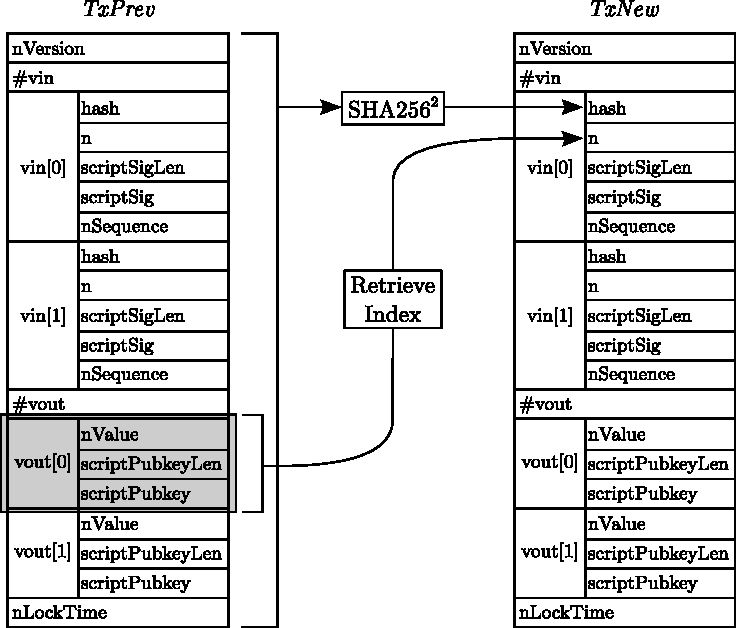
\includegraphics[scale=0.975]{Images/Transaction2In2Out.pdf}
 \caption{Signature Computation - Initial State} \label{fig:Signature-InitState}
\end{figure}
\vspace{-5pt}

\noindent
In the following the various signature types will be discussed in detail. The depiction in Fig. \ref{fig:Signature-InitState} shows the initial state of a sample transaction which will be used to illustrate the process. The signature will be performed for the first transaction input of the transaction \emph{TxNew}, which references the first output of a past transaction \emph{TxPrev}.

\clearpage
\subsection*{SIGHASH\_ALL}
The default signature hash type \emph{SIGHASH\_ALL} represents the simplest of the three base types. It signs the complete transaction, including all the transactions inputs and outputs, with the exception of the signature script fields. The coverage of the signature is illustrated below in Fig. \ref{fig:SigHash-All} with grey fields.

\begin{figure}[ht!]
 \centering
 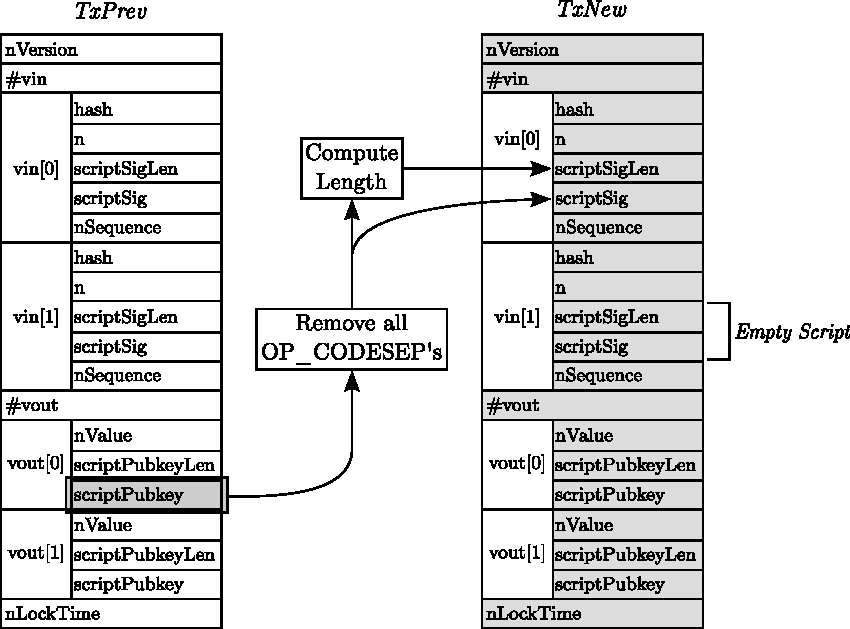
\includegraphics[scale=0.975]{Images/SIGHASH_ALL.pdf}
 \caption{Signature Computation - SIGHASH\_ALL} \label{fig:SigHash-All}
\end{figure}

\noindent
Before the signature is computed, several temporary changes are made to the transaction:
\begin{enumerate}[label=\alph*), leftmargin=1cm]
\item The signature script of the currently signed input is replaced with the public key script, excluding all occurences of \texttt{OP\_CODESEPARATOR} in it, of the referenced transaction output.
\item The signature scripts of all other inputs are replaced with empty scripts.
\end{enumerate}


\clearpage
\subsection*{SIGHASH\_SINGLE}
In the second signature hash type \emph{SIGHASH\_SINGLE} all transaction inputs and the transaction output corresponding to the currently signed input is signed. The coverage of the signature is illustrated below in Fig. \ref{fig:SigHash-Single} with grey fields.

\begin{figure}[ht!]
 \centering
 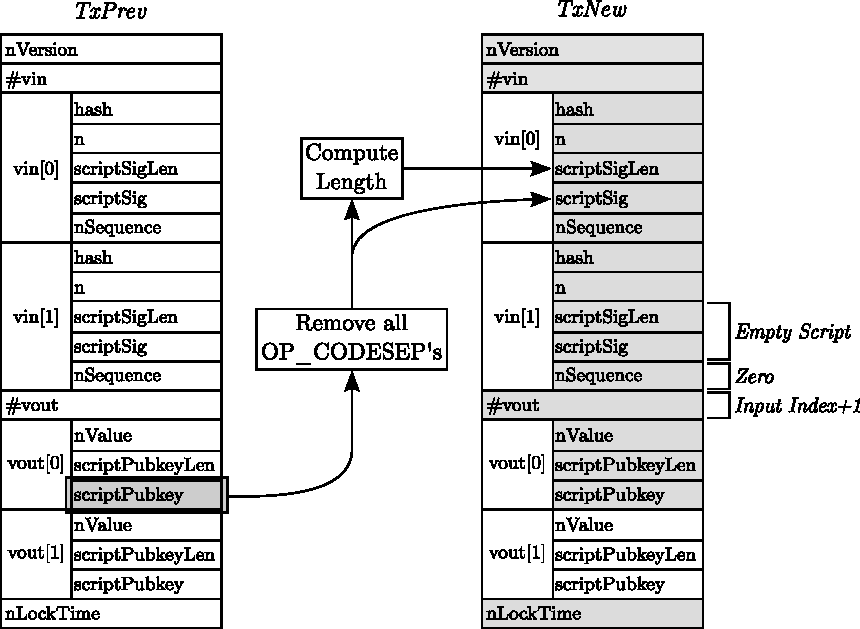
\includegraphics[scale=0.975]{Images/SIGHASH_SINGLE.pdf}
 \caption{Signature Computation - SIGHASH\_SINGLE} \label{fig:SigHash-Single}
\end{figure}

\noindent
Before the signature is computed, several temporary changes are made to the transaction:
\begin{enumerate}[label=\alph*), leftmargin=1cm]
\item The signature script of the currently signed input is replaced with the public key script, excluding all occurences of \texttt{OP\_CODESEPARATOR} in it, of the referenced transaction output.
\item For all the remaining transaction inputs:\vspace{5pt}
\begin{itemize}
\item[-] The signature scripts are replaced with empty scripts.
\item[-] The sequence number is set to zero.
\end{itemize}
\item The number of transaction outputs is set to the currently signed transaction input index plus one.
\item All transaction outputs up to the currently signed one are emptied.
\end{enumerate}


\clearpage
\subsection*{SIGHASH\_NONE}
In the third signature hash type \emph{SIGHASH\_NONE} all transaction inputs and none of the transaction outputs are signed. The coverage of the signature is illustrated below in Fig. \ref{fig:SigHash-None} with grey fields.

\begin{figure}[ht!]
 \centering
 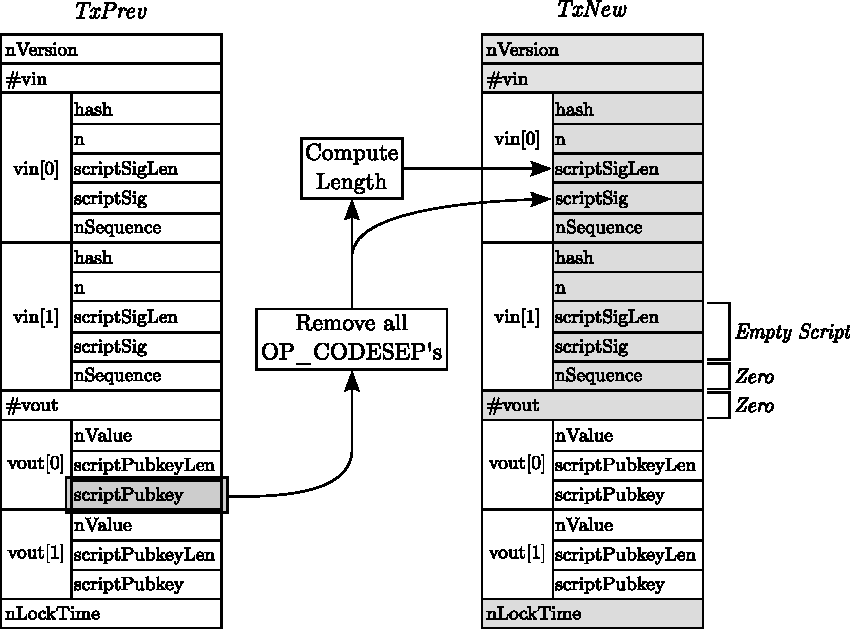
\includegraphics[scale=0.975]{Images/SIGHASH_NONE.pdf}
 \caption{Signature Computation - SIGHASH\_NONE} \label{fig:SigHash-None}
\end{figure}

\noindent
Before the signature is computed, several temporary changes are made to the transaction:
\begin{enumerate}[label=\alph*), leftmargin=1cm]
\item The signature script of the currently signed input is replaced with the public key script, excluding all occurences of \texttt{OP\_CODESEPARATOR} in it, of the referenced transaction output.
\item For all the remaining transaction inputs:\vspace{5pt}
\begin{itemize}
\item[-] The signature scripts are replaced with empty scripts.
\item[-] The sequence number is set to zero.
\end{itemize}
\item The number of transaction outputs is set to zero.
\item All transaction outputs are removed.
\end{enumerate}


\clearpage
\subsection*{SIGHASH\_ANYONECANPAY}
The \emph{SIGHASH\_ANYONECANPAY} modifier is used in conjunction with a base type and affects the signature coverage of transaction inputs. It is used to only cover the currently signed input by the signature. For example, the transaction depicted in Fig. \ref{fig:SigHash-Anyone} illustrates that the second transaction input is excluded from the signature.

\begin{figure}[ht!]
 \centering
 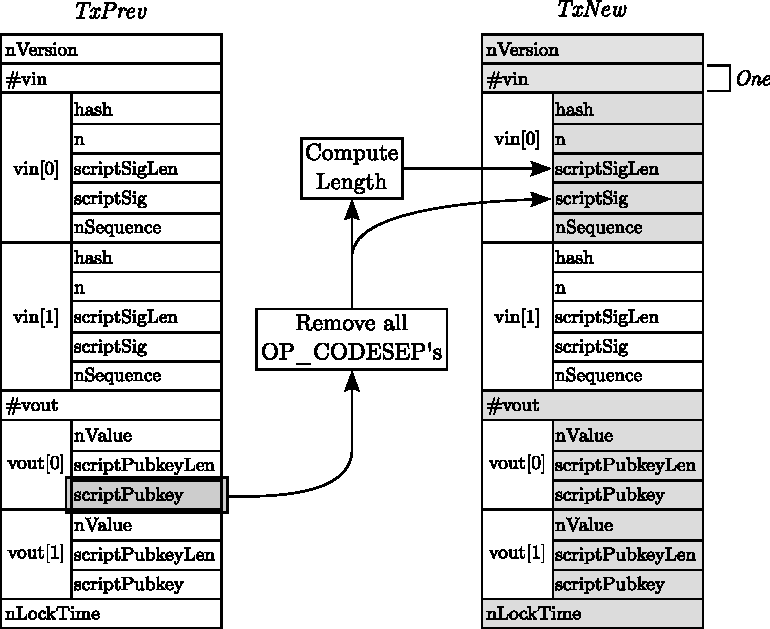
\includegraphics[scale=0.975]{Images/SIGHASH_ANYONECANPAY.pdf}
 \caption{Signature Computation - SIGHASH\_ALL\textbar SIGHASH\_ANYONECANPAY} \label{fig:SigHash-Anyone}
\end{figure}

\noindent
In addition to the changes performed by the base hash type, the following temporary changes are made before the signature is computed:
\begin{enumerate}[label=\alph*), leftmargin=1cm]
\item The number of transaction inputs is set to one.
\item All transaction inputs, except for the currently signed one, are removed.
\end{enumerate}

\clearpage
\subsection*{Finalization}
Once the transaction type has been chosen and the hash type dependent modifications have been applied, the actual signature is computed. This is done as follows - first, the hash type is appended to the transaction, then the signature itself is computed and finally the hashtype is appended to it. The ECDSA signature is computed using double-SHA256 and the secp256k1 elliptic curve as parameters. The appended hashtype signals the verifying party what hash type was applied.

\begin{figure}[ht!]
 \centering
 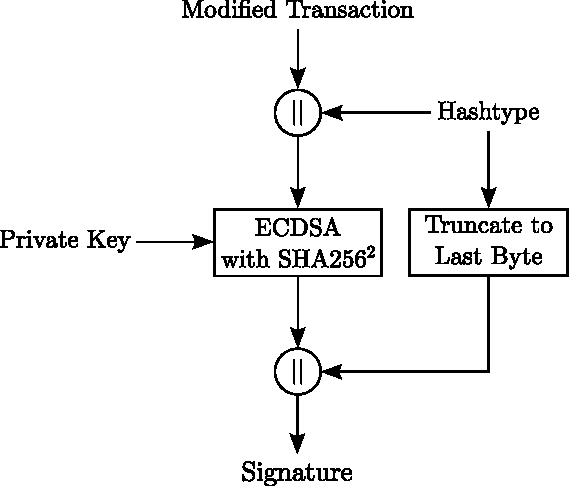
\includegraphics[scale=0.9]{Images/Signature-Finalization.pdf}
 
 \vspace{5pt}
 \caption{Signature Computation - Finalization} \label{fig:SigFin-SighashAll}
\end{figure}

\clearpage
\section{Blockchain} \label{sec:Blockchain}

\subsection{Structure} \label{sec:BlockchainStructure}
The blockchain is a record of all transactions that have occured in the Bitcoin system and is shared by every node in it. Its main purpose is to infer spending for all transaction outputs. The novelty of Bitcoin lies, among other things, in how the blockchain is structured in order to guarantee chronological ordering of transactions and prevent double-spending in a distributed network.

As described in Sect. \ref{sec:Blocks}, every block in the blockchain refers to the hash of a previous block. This imposes a chronological order on blocks and therefore transactions as well, since it is not possible to create a valid hash of the previous block header prior to its existence.

Furthermore, each block includes the solution to a proof-of-work puzzle of a certain difficulty. The computational power involved in solving the proof-of-work puzzle for each block is used as a voting scheme to enable all nodes in the network to collectively agree on a version of the blockchain. Nodes collectively agree on the blockchain that involved the highest accumulated computational effort to be created. Thus, modifying a block in the chain would require an adversary to recompute proof-of-work puzzles of equal or greater computational effort than the ones from that block up until the newest block. In order to achieve that, the adversary would have to computationally outperform the majority of the network, which is considered infeasible.
\begin{figure}[ht!]
 \centering
 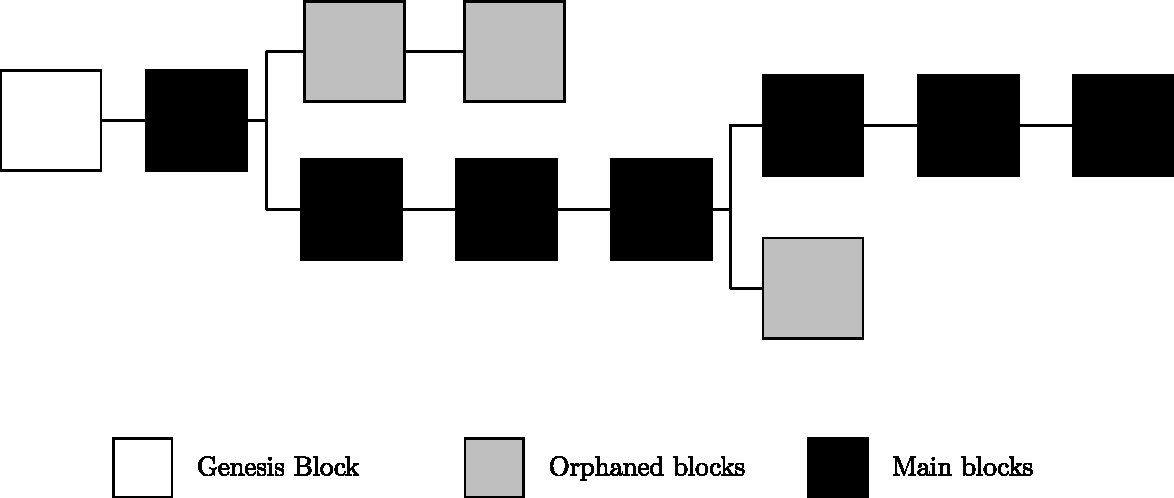
\includegraphics[scale=0.6]{images/Blockchain.pdf}
 \caption{Blockchain}
 \label{figure:Blockchain}
\end{figure}

\noindent
Clearly, since nodes in the network compete in a randomized process to successfully solve the proof-of-work puzzle and gain a reward, there is a chance that two different blocks are mined simultaneously and the chain forks. In this case nodes will accept whichever block they have received first and continue building the chain upon that block. If another block is found, then the branch that was used will become the main blockchain. If this happens, all valid transactions within the shorter chain are re-added to the pool of queued transactions. The resulting structure resembles what is depicted in Fig. \ref{figure:Blockchain}, the white block being the first block ever mined, also referred to as the genesis block, the black chain representing the main chain and grey blocks being orphans due to forking.

\subsection{Mining} \label{sec:Mining}

\subsubsection*{Procedure}
The process of finding a valid block is called \emph{mining} whereas nodes that participate in that process are called \emph{miners}. As described in \cite{Clark_BitcoinInternals}, mining nodes perform the following steps in an endless loop:

\begin{enumerate}[label=\arabic*), leftmargin=1cm]
\item Collect all broadcasted transactions and validate whether they satisfy the miner's self-defined policy. Typically, a transaction includes a transaction fee that functions as an incentive for the miner to include it in the block. However, if it does not, then it is up to the miner to decide what to do with it.
\item Verify all transactions that are to be included in the block. Transactions are verified as described in Sect. \ref{sec:Script} and it is checked whether their inputs have been previously spent.
\item Select the most recent block on the longest path in the blockchain, i.e. the path that involves most accumulated computational effort, and insert the hash of the block header into the new block.
\item Solve the proof-of-work problem as described below and broadcast the solution. Should another node solve the proof-of-work problem before, then the block is first validated - the proof-of-work solution is checked and all transactions included in the block are verified. If it passes these controls then the cycle is repeated. Note that if there are transactions that have not been included in the new block then they are saved and included in the next cycle.
\end{enumerate}


\subsubsection*{Proof-of-Work}
During mining a miner attempts to find a block header whose double-SHA256 hash lies below the target value $T$. In order to succeed he needs a certain degree of freedom in the block header that allows him to compute various hashes without interfering with its semantics. Hence, two fields are used as a source of randomness - the nonce field (\textit{nNonce}) in the block header itself and the coinbase field (\textit{coinbase}) in the coinbase transaction, which indirectly changes the Merkle root (\textit{HashMerkleRoot}) in the block header. The process of finding a proof-of-work can then be divided into three steps:

\begin{enumerate}[label=\arabic*), leftmargin=1cm]
\item Set the nonce field and the coinbase field to values of one's choosing.
\item Compute the hash of the block header as
\begin{equation}
SHA256^{2}(nVersion||HashPrevBlock||HashMerkleRoot||nTime||nBits||nNonce)
\label{eqn:HashBlock}
\end{equation}
\item Reverse the byte order of the computed hash and check whether its value $\mathit{H}$ lies below the current target value $\mathit{T}$ (stored in compact format in the \textit{nBits} field):
\begin{equation}
H \leq T
\end{equation}

\end{enumerate}

\noindent
This process is repeated for various values of \textit{nNonce} and \textit{coinbase} until a valid solution is found. Typically, for efficiency reasons, all possible values of the nonce field are evaluated before changes to the coinbase field are made.



%%%----------------------------------------------------------
\renewcommand*{\thesection}{\appendixname~\Alph{section}}%
\addtocontents{toc}{\protect\vskip15pt}


\titlecontents{section}
  [7em]{}
  {\bfseries\contentslabel{6em}\vspace{6pt}}
  {\hspace*{0em}}
  {\titlerule*[0.422pc]{.}\contentspage}

%%%----------------------------------------------------------
\begin{appendices}

\section{Data types} \label{sec:DataTypes}

\subsection*{General data types}

\vspace{4pt}
\begin{center}
	\begin{tabularx}{\textwidth}{| c | c | X |}
		\hline
		\textbf{Type} & \textbf{Size (bytes)} & \textbf{Description} \\ \hline \hline
		int & 4 & Signed integer in little-endian. \\ \hline
		uint & 4 & Unsigned integer in little-endian. \\ \hline
		uint8\_t & 1 & Unsigned integer. \\ \hline
		uint16\_t & 2 & Unsigned integer in little-endian. \\ \hline
		uint32\_t & 4 & Unsigned integer in little-endian. \\ \hline
		uint64\_t & 8 & Unsigned integer in little-endian. \\ \hline
		uint160 & 20 & Unsigned integer array uint32\_t[] of size 5. \newline Used for storing RIPEMD160 hashes as a byte array.\\ \hline
		uint256 & 32 & Unsigned integer array uint32\_t[] of size 8. \newline Used for storing SHA256 hashes as a byte array.\\ \hline
	\end{tabularx}
\end{center}
\vspace{10pt}

\subsection*{Variable length integers (VarInt)}
Integers in Bitcoin can be encoded depending on the value in order to save space. Variable length integers always precede vectors of a type of data that may vary in length. An overview of the different variable length integes is depicted below.

\begin{center}
\begin{tabular}{| C{0.3\linewidth} | C{0.1\linewidth} | C{0.5\linewidth} |}
	\hline
	\textbf{Value interval} & \bigcell{c}{\textbf{Size} \\ \textbf{(bytes)}} & \textbf{Format} \\ \hline \hline
    $\left[{0,2^{8}-3}\right)$ & 1 & uint8\_t \\ \hline
	$\left[2^{8}-3, 2^{16}\right)$ & 3 & 0xFD followed by the value as uint16\_t \\ \hline
	$\left[2^{16}, 2^{32}\right)$ & 5 & 0xFE followed by the value as uint32\_t \\ \hline
	$\left[2^{32}, 2^{64}\right)$ & 9 & 0xFF followed by the value as uint64\_t \\ \hline
\end{tabular}
\end{center}


\clearpage
\section{Calculations} \label{sec:Calculations}
\subsubsection*{Dust Transactions}~\\
A transaction is defined as ``dust'', if any of the transaction outputs spends more than 1/3rd of its value in transaction fees. More precisely, a transaction is considered ``dust'' if any of its transaction outputs satisfies the inequality

\begin{equation}
\dfrac{\dfrac{TxFeeRate}{1000}*(TxOutSize + 148)}{nValue} > \dfrac{1}{3}
\end{equation}

\noindent
where {\tt nValue} is the transaction output value, {\tt TxOutSize} is the transaction output size in bytes and {\tt TxFeeRate} is the transaction fee rate in Satoshi per kB. Given that the default transaction fee rate currently lies at 1000 Satoshi per kB and that the size of a typical transaction output is 34 bytes, the resulting minimal transaction output value is 546 Satoshi.


%\clearpage
%\section{Script Commands} \label{sec:ScriptCommands}
%
%\subsection*{Constants}
%\begin{center}
%	\begin{tabular}{| C{0.225\linewidth} | C{0.125\linewidth} |
%						>{\em}C{0.125\linewidth} | >{\em}C{0.125\linewidth} | C{0.35\linewidth} |}
%		\hline
%		\textbf{Word} & \textbf{Opcode} & \textbf{Input} & \textbf{Output} & \textbf{Description} \\ \hline \hline
%		
%		OP\_0, OP\_FALSE & 0x00 &
%		None & Empty value &
%		An empty array of bytes is pushed onto the stack.\\ \hline
%	
%		N/A	& 0x01-0x4B	&
%		(Special) &	Data &
%		The next \emph{opcode} bytes is data to be pushed onto the stack.\\ \hline
%		
%		OP\_PUSHDATA1 &	0x4C &
%		(Special) & Data &
%		The next byte contains the number of bytes to be pushed onto the stack.\\ \hline
%		
%		OP\_PUSHDATA2 & 0x4D &
%		(Special) & Data &
%		The next two bytes contain the number of bytes to be pushed onto the stack.\\ \hline
%		
%		OP\_PUSHDATA4 &	0x4E &
%		(Special) & Data &
%		The next four bytes contain the number of bytes to be pushed onto the stack.\\ \hline
%		
%		OP\_1NEGATE	& 0x4F &
%		None & -1 &
%		The number -1 is pushed onto the stack.\\ \hline
%		
%		OP\_1, OP\_TRUE & 0x51 &
%		None & 1 &
%		The number 1 is pushed onto the stack.\\ \hline
%		
%		OP\_2-OP\_16 & 0x52-0x60 &
%		None & 2-16 &
%		The number in the word name (2-16) is pushed onto the stack.\\ \hline
%	
%	\end{tabular}
%\end{center}
%
%\subsection*{Crypto}
%\begin{center}
%	\begin{tabular}{| C{0.225\linewidth} | C{0.125\linewidth} |
%						>{\em}C{0.125\linewidth} | >{\em}C{0.125\linewidth} | C{0.35\linewidth} |}
%		\hline
%		\textbf{Word} & \textbf{Opcode} & \textbf{Input} & \textbf{Output} & \textbf{Description} \\ \hline \hline
%		
%		OP\_HASH160	& 0xA9 &
%		Data & Hash &
%		The top stack element is hashed twice: first with SHA-256 and then with RIPEMD-160.\\ \hline
%		
%		OP\_CHECKSIG & 0xAC &
%		Signature Pubkey & True / False	&
%		The transaction is hashed and the signature is verified for this hash and public key. The result is pushed onto the stack.\\ \hline
%		
%		OP\_CHECK- MULTISIG &	0xAE &
%		OP\_0 sig1 ... m pub1 ... n & True / False &
%		For each signature and public key pair, OP\_CHECKSIG is executed. The result is pushed onto the stack.\\ \hline
%
%	\end{tabular}
%\end{center}
%\vspace{10pt}
%
%\subsection*{Other}
%\begin{center}
%	\begin{tabular}{| C{0.225\linewidth} | C{0.125\linewidth} |
%						>{\em}C{0.125\linewidth} | >{\em}C{0.125\linewidth} | C{0.35\linewidth} |}
%		\hline
%		\textbf{Word} & \textbf{Opcode} & \textbf{Input} & \textbf{Output} & \textbf{Description} \\ \hline \hline
%		
%		OP\_DUP & 0x76 &
%		Data & Data Data &
%		Duplicates the top stack item.\\ \hline
%		
%		OP\_EQUAL & 0x87 &
%		Data1 Data2 & True / False &
%		Returns \emph{true} if the top two stack elements are exactly equal, \emph{false} otherwise. The result is pushed onto the stack.\\ \hline
%
%		OP\_EQUAL- VERIFY & 0x88 &
%		Data1 Data2 & True / False & 
%		Same as OP\_EQUAL, but marks transaction as invalid if it fails.\\ \hline
%
%		OP\_RETURN & 0x6A &
%		None & None &
%		Marks transaction as invalid.\\ \hline
%
%	\end{tabular}
%\end{center}
%\vspace{10pt}

\end{appendices}


%%%----------------------------------------------------------
% Bibliography
%%%----------------------------------------------------------
\clearpage
\fancypagestyle{plain}{% new plain style
  \fancyhf{}% Clear header/footer
  \fancyhead[LE,RO]{\bfseries\thepage}
  \fancyhead[LO]{\bfseries\bibmark} % Odd pages, section name printed
  \fancyhead[RE]{\bfseries\titlemark}% Right header
}
\pagestyle{plain}
\bibliographystyle{plain}
\bibliography{literature}

\end{document}
